%(BEGIN_QUESTION)
% Copyright 2007, Tony R. Kuphaldt, released under the Creative Commons Attribution License (v 1.0)
% This means you may do almost anything with this work of mine, so long as you give me proper credit

Her vises responsen til en prosess på en serie trinnendringer i regulatorutgangen (alle gjort mens regulatoren stod i ``manuell'' modus). Hva kan du, basert på observasjonene, fastslå om prosessen og tilhørende instrumentering?

$$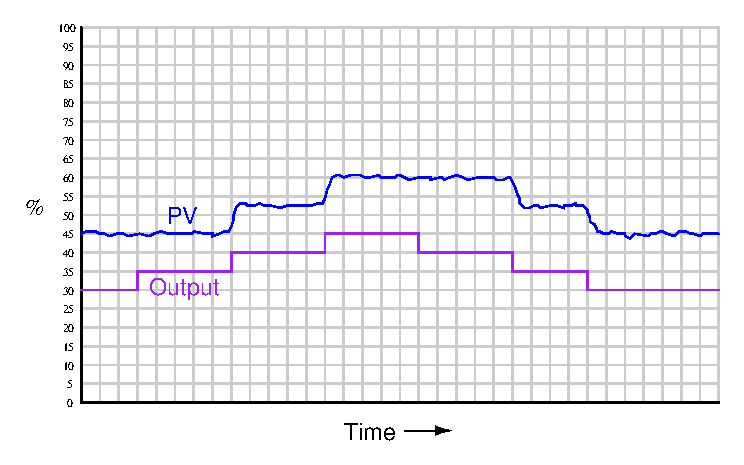
\includegraphics[width=15.5cm]{i01649x01.eps}$$

\underbar{file i01649}
%(END_QUESTION)





%(BEGIN_ANSWER)

Dette plottet av PV-respons for flere trinnendringer i utgangen viser at prosessen har betydelig {\it hysterese}. Hvis dette er en prosess regulert av ventil, ville jeg mistenke at ventilen har betydelig ``stiction'' og/eller slark i en mekanisk kobling.

Legg merke til at den første trinnendringen oppover i utgangen ikke har noen målbar effekt på prosessvariabelen. Men ved andre og tredje trinnendring oppover responderer prosessvariabelen umiddelbart med sprang oppover. Tilsvarende gir den første trinnendringen nedover i utgangen ingen målbar effekt på prosessvariabelen. Prosessen responderer derimot raskt på andre og tredje trinnendring nedover. Oppsummert ser vi ingen effekt ved første retningsendring i utgangen. Dette er typisk for {\it hysterese}, uansett hvor i systemet den sitter. Den mest sannsynlige kilden til denne hysteresen er reguleringsventilen (stiction).

%(END_ANSWER)





%(BEGIN_NOTES)

%INDEX% Control, PID tuning: step change (output) revealing hysteresis

%(END_NOTES)
